\documentclass[ngerman,
color=3b,
% dark_mode, 
load_common, % Loads a list of commonly used Packages
boxarc,
main,
% manual_term,
% solution=true,
tikz,
border=3mm
]{article}



\usepackage{lmodern}

\usepackage{graphicx}
\usepackage[margin=2cm]{geometry}
\usepackage[utf8]{inputenc}
\usepackage[table,xcdraw,svgnames]{xcolor}
\usepackage{amsmath,amsfonts,amsthm,amssymb} %Math & symbols
\usepackage{booktabs}
\usepackage[hidelinks]{hyperref} % For hyperlinks, automatically created for table of contents


\usepackage[protrusion=true,expansion=true]{microtype}

%-----------------------------------
% Table of Contents
%-----------------------------------
\usepackage{tocloft}
\addtolength{\cftsecnumwidth}{40pt} % Set width between title of section and number of section
\renewcommand{\contentsname}{\vspace{-20pt}}


%-----------------------------------
% Algorithms
%-----------------------------------
\usepackage{listings}
\definecolor{codegreen}{rgb}{0,0.6,0}
\definecolor{codegray}{rgb}{0.5,0.5,0.5}
\definecolor{codepurple}{rgb}{0.58,0,0.82}
\definecolor{backcolour}{rgb}{0.95,0.95,0.92}

\lstdefinestyle{mystyle}{
    backgroundcolor=\color{backcolour},   
    commentstyle=\color{codegreen},
    keywordstyle=\color{magenta},
    numberstyle=\tiny\color{codegray},
    stringstyle=\color{codepurple},
    basicstyle=\ttfamily\footnotesize,
    breakatwhitespace=false,         
    breaklines=true,                 
    captionpos=b,                    
    keepspaces=true,                 
    numbers=left,                    
    numbersep=5pt,                  
    showspaces=false,                
    showstringspaces=false,
    showtabs=false,                  
    tabsize=2
}

\lstset{style=mystyle}

\usepackage[
    linesnumbered,
    lined,
    %boxed,
    commentsnumbered,
    ]{algorithm2e}%Algortihms
    
\SetAlgoNlRelativeSize{-1}

\usepackage{algpseudocode}
\usepackage{algorithmicx}

\SetKw{KwContinue}{\color{blue}continue}
\SetKw{KwBreak}{\color{red}break}
\SetKw{KwDownTo}{down to}
\SetKw{KwAnd}{\color{teal}and}
\SetKw{KwOr}{\color{teal}or}
\SetKw{KwError}{\color{red}error}
\SetKwProg{Fn}{\color{MediumSeaGreen}Function}{:}{}
\SetKwProg{Cl}{\color{MediumSeaGreen}Class}{:}{}

%-----------------------------------
% Trees, Skip-Lists etc.
%-----------------------------------
\usepackage{tikz}
\usepackage{tkz-graph}
\usetikzlibrary{trees}
\usetikzlibrary{shapes.geometric}
\usetikzlibrary{calc}
\usetikzlibrary{arrows}
\usetikzlibrary{chains}

%-------------------------------------
% Captions
%-------------------------------------
\usepackage[hang, small,labelfont=bf,up,textfont=it,up,labelformat=empty]{caption}
% \captionsetup[figure]{name=Skip-List}

\usepackage{caption}
\usepackage[]{sectsty}
\usepackage{titlesec}
%------------------------
% Footer and Header
%------------------------
\usepackage[]{fancyhdr} % For footers and header
\pagestyle{fancy}
\usepackage[]{lastpage} %For page reference: Page x out of y

\lhead{} % Left Header
\chead{} % Centre Header
\rhead{} % Right Header

\lfoot{} % Left Footer
\cfoot{} % Centre Footer
\rfoot{\footnotesize Seite \thepage\ von \pageref{LastPage}} % Right Footer - Page Reference

\renewcommand{\headrulewidth}{0.0pt} % Sets size of header rule - here its not visible 
\renewcommand{\footrulewidth}{0.4pt} % Sets size of footer rule
%----------------------------------------------
% Title
%----------------------------------------------
\usepackage{titling}
\newcommand{\HorRule}{\color{Black} \rule{\linewidth}{2pt}}
\newcommand{\TitleRule}{\color{Green} \rule{\linewidth}{15pt} \vspace{-90pt}\linebreak \HorRule \linebreak}
%\newcommand{\TitleRule}{\color{Green} \titlerule[15pt] \color{White} \titlerule[7pt] \color{Black} \titlerule[2pt]}
\newcommand{\SectionHorRule}{\color{Black} \rule{\linewidth}{1pt}}

\pretitle{\vspace{-80pt} \fontsize{30}{50} \usefont{OT1}{phv}{b}{n} \TitleRule \color{Black}} % Horizontal rule before the title
	
	\title{AuD - Zusammenfassung} % The title
	
	\posttitle{\vskip 0.5em} % Whitespace under the title

\preauthor{\begin{flushleft}\large \lineskip 0.5em \fontsize{15}{0} \usefont{T1}{phv}{b}{n} \color{Black}} % Author font configuration
	
	\author{Moritz Gerhardt } % Name
	
	\postauthor{% Anything you might want to add
		\par\end{flushleft}} % Horizontal rule after the title

\date{} % Add date or leave empty to not show any date !!!\today

%-----------------------------
% Section Style
%-----------------------------

\newcommand{\SectionFont}{\LARGE\bfseries}
\titleformat{\section} % Type of heading to format
%[] % Shape
{\color{Green} \titlerule[15pt] \color{White} \titlerule[7pt] \color{Black} \titlerule[2pt] \SectionFont} % Format
{\thesection} % Label
{1em} % Seperator
{\SectionFont} % Before-Code
[{\titlerule[2pt]}] % After-Code

\newcommand{\SubSectionFont}{\large\bfseries}
\titleformat{\subsection} % Type of heading to format
%[] % Shape
{\SubSectionFont} % Format
{\thesubsection} % Label
{1em} % Seperator
{\SubSectionFont} % Before-Code
[{\titlerule[1pt]}] % After-Code

\renewcommand{\thesection}{Sektion \space \arabic{section}}
\renewcommand{\thesubsection}{\arabic{section}.\arabic{subsection}}
\renewcommand{\thesubsubsection}{\arabic{section}.\arabic{subsection}\space(\alph{subsubsection})}

\usepackage{parskip} % Removes the indentation of the first line of new section

\begin{document}

%\thispagestyle{fancy}
\maketitle
\section{Inhalt}
\tableofcontents

\newpage

\section{Was ist ein Algorithmus?}
Ein Algorithmus beschreibt eine Handlungsvorschrift zur Umwandlung von Eingaben in eine Ausgabe.\\
Dabei sollte ein Algorithmus im allgemeinen folgende Vorraussetzungen erfüllen:
\begin{enumerate}
    \item Bestimmt:
    \begin{itemize}
        \item Determiniert: Bei gleicher Eingabe liefert der Algortihmus gleiche Ausgabe. \\$\implies$ Ausgabe nur von Eingabe abhängig, keine äußeren Faktoren.
        \item Determinismus: Bei gleicher Eingabe läuft der Algorithmus immer gleich durch die Eingabe. \\$\implies$ Gleiche Schritte, Gleiche Zwischenstände.
    \end{itemize}
    \item Berechenbar:
    \begin{itemize}
        \item Finit: Der Algorithmus ist als endlich definiert. (Theoretisch)
        \item Terminierbar: Der Algorithmus stoppt in endlicher Zeit. (Praktisch)
        \item Effektiv: Der Algorithmus ist auf Maschine ausführbar.
    \end{itemize}
    \item Andwendbar:
    \begin{itemize}
        \item Allgemein: Der Algorithmus ist für alle Eingaben einer Klasse anwendbar, nicht nur für speziellen Fall.
        \item Korrekt: Wenn der Algorithmus ohne Fehler terminiert, ist die Ausgabe korrekt.
    \end{itemize}
\end{enumerate}

\newpage
\section{Laufzeitanalyse}
\subsection{O Notation}
Die O-Notation wird grundsätzlich für \textit{Worst-Case} Laufzeiten verwerdendet. Sie gibt also eine obere Schranke an, die der Algorithmus im schlechtesten Fall erreicht. Dabei wird oft zwischen Big O-Notation und Little o-Notation unterschieden. 
Ein Graph zur Repräsentation der O-Notation ist hier zu sehen:
\begin{center}
    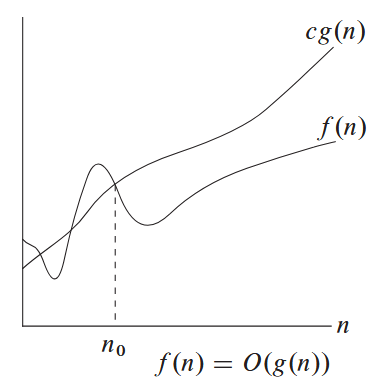
\includegraphics[scale=0.6]{Pics/ONotation.png}
\end{center}

\subsubsection{Big-O Notation}
Mathematische Definition: 
\begin{center}
    $O(g(n)) = \exists c \in \mathbb{R}_{>0}, n_0 \in \mathbb{N}, \forall n \geq n_0:  0 \leq f(n) \leq c \cdot g(n)$
\end{center}
Es existieren Konstanten $c$ in den positiven reelen Zahlen und $n_0$ in den natürlichen Zahlen, sodass für alle $n \geq n_0$ gilt, dass  $f(n)$ \color{teal}$\geq$ \color{black} 0 und $f(n)$ \color{red}$\leq$ \color{black}$c \cdot g(n)$. \\
Das bedeutet, dass die Funktion $f(n)$ für $n \to \infty$ den gleichen Wachstumsfaktor hat wie die Funktion $g(n)$.
Einfache Berechnung findet wie folgt statt (anhand vom Beispiel $f(n) = 5n^2 + 2n$):
\begin{enumerate}
    \item Finde den Term mit dem höchsten Wachstumsfaktor ($5n^2$)
    \item Konstanten werden weggelassen ($n^2$)
    \item Demnach ist $f(n) = O(n^2)$
\end{enumerate}
Dies kann man dann im Rückschluss so anwenden:
Um die Konstanten $c$ und $n_0$ zu finden, wird die obige gleichung benutzt:
\begin{enumerate}
    \item Simplifiziere die Ungleichung $5n^2 + 2n \leq c \cdot n^2$ zu $5 + \frac{2}{n} \leq c$
    \item Da $n \geq n_0$ kann man die Gleichung für $n \geq 1$ auflösen um die Konstanten $c$ und $n_0$ zu finden. \\
    $\implies$ $5 + \frac{2}{1} = 7 \leq c$ $\implies$ $c \geq 7$
    \item Dementsprechend kann man dann die Konstanten $c = 7$ und $n_0 = 1$ auswählen.
\end{enumerate}

\newpage
\subsubsection{Little-o Notation}
Mathematische Notation:
\begin{center}
    $O(g(n)) = \exists c \in \mathbb{R}_{>0}, n_0 \in \mathbb{N}, \forall n \geq n_0:  0 \leq f(n) < c \cdot g(n)$
\end{center}
Es existieren Konstanten $c$ in den positiven reelen Zahlen und $n_0$ in den natürlichen Zahlen, sodass für alle $n \geq n_0$ gilt, dass  $f(n)$ \color{teal}$\geq$ \color{black} 0 und $f(n)$ \color{red}$<$ \color{black}$c \cdot g(n)$. Little-o Notation unterscheidet sich also von Big-O Notation nur oberen Schranke. Während bei Big-O der Wachstumsfaktor beider Funktion gleich sein kann ($f(n) = c \cdot g(n)$), gilt bei Little-o, dass der Wachstumsfaktor der Funktion $f(n)$ kleiner ist als der Wachstumsfaktor der Funktion $g(n)$. \\
Einfache Berechnung findet analog zu Big-O wie folgt statt (anhand vom Beispiel $f(n) = 5n^2 + 2n$):
\begin{enumerate}
    \item Finde den Term mit dem höchsten Wachstumsfaktor ($5n^2$)
    \item Konstanten werden weggelassen ($n^2$)
    \item Demnach ist $f(n) = o(n^2)$
\end{enumerate}
Hier muss allerdings noch geprüft werden, ob der Wachstumsfaktor der Funktion $f(n)$ kleiner ist als der Wachstumsfaktor der Funktion $g(n)$. Wenn ja, ist die Little-o Notation korrekt für $g(n)$. \\
Um zu zeigen, dass $f(n) = o(g(n))$:
\begin{enumerate}
    \item Finde den Limes des simplifizierten Ausdrucks $\frac{f(n)}{g(n)}$, der die Wachstumsrate der Funktion $f(n)$ zur Wachstumsrate der Funktion $g(n)$ vergleicht.
    \begin{itemize}
        \item $\lim_{n \to \infty} \frac{f(n)}{g(n)} = \lim_{n \to \infty} \frac{5n^2 + 2n}{n^2} = \lim_{n \to \infty} 5 + \frac{2}{n} = 5$
        \item Da $\frac{2}{n}$ für $n \to \infty$ bei 0 konvergiert.
    \end{itemize}
    \item Da der Limes $\not= 0$ ist, bedeutet das, dass der Wachstum von $f(n)$ nicht geringer ist als der von $g(n)$. Deshalb müssen wir ein Polynomgrad hochgehen, weswegen $f(n) = o(n^3)$ sein muss. 
    \item Um nun die Konstanten $c$ und $n_0$ zu finden müssen wir einfach $\frac{f(n)}{g(n)}$ auflösen
    \begin{itemize}
        \item $\frac{5n^2 + 2n}{n^3} < c$
        \item $\frac{5}{n} + \frac{2}{n^2} < c$
        \item $\frac{5}{n} < c$, da $\frac{2}{n^2}$ für $n \to \infty$ schneller abfällt als $\frac{5}{n}$
        \item Für $c = 1$ muss dann $n_0 > 5$ sein und kann somit als $n_0 = 6$ gewählt werden.
    \end{itemize}
\end{enumerate}

\newpage
\subsection{$\Omega$\space Notation}
Ähnlich zur O Notation, allerdings geht es hier um den \textit{Best-Case} also minimale Anzahl der Schritten, die ein Algorithmus ausführt.
\begin{center}
    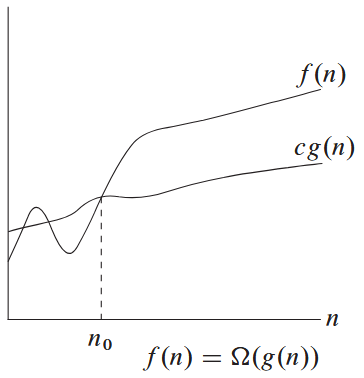
\includegraphics[scale=0.6]{Pics/OmegaNotation.png}
\end{center}
Wird auch wieder in $\Omega$ und $\omega$ aufgeteilt, die sich nur darin unterscheiden, wie strikt die Grenze ist.
\subsubsection{$\Omega$ Notation}

\newpage 
\section{Sortieren}
\subsection{Sortierproblem}
Sortieralgorithmen sind die wohl am häufigsten verwendeten Algorithmen. Hierbei wird als Eingabe eine Folge von Objekten gegeben, die nach einer bestimmten Eigenschaft sortiert werden. Der Algorithmus soll die Eingabe in der richtigen Reihenfolge (nach einer bestimmten Eigenschaft) zur Ausgabe umwandeln. Es wird hierbei meist von einer total geordneten Menge ausgegangen. (Alle Elemente sind miteinander vergleichbar). \\
Eine Totale Ordnung wie folgt definiert:
\begin{center}
    Eine Relation $\leq$ auf $M$ ist eine totale Ordnung, wenn:
    \begin{itemize}
        \item Reflexiv: $\forall x \in M: x \leq x$ \\
        (x steht in Relation zu x)
        \item Transitiv: $\forall x,y,z \in M: x \leq y \wedge y \leq z \implies x \leq z$ \\
        (Wenn x in Relation zu y steht und y in Relation zu z steht, so folgt, dass x in Relation zu z steht)
        \item Antisymmetrisch: $\forall x,y \in M: x \leq y \wedge y \leq x \implies x = y$ \\
        (Wenn x in Relation zu y steht und y in Relation zu x steht, so folgt, dass x = y)
        \item Totalität: $\forall x,y \in M: x \leq y \vee y \leq x$ \\
        (Alle Elemente müssen in einer Relation zueinander stehen)
    \end{itemize}
\end{center}
\newpage
\subsection{Insertion Sort}
\lstinputlisting[language=Java]{Code/InsertionSort.java}

Prinzip: Die Eingabe wird von links nach rechts durchlaufen. Dafür wird für jedes Element startend bei i = 1 der Array von i bis 0 nach links durchlaufen, bis 0 erreicht ist oder key-Wert größer gleich dem i-ten Element ist. \\ 
Während des durchlaufens nach links werden die Elemente so nach Rechts geschoben, so dass eine Einfügespalte ensteht. Nach dem Ende dieses Durchgangs ist der Spalt bei der position, bei der der Wert eingefügt werden soll. \\
Dies wird dann wiederholt, bis für alle i der Array durchlaufen ist.

\newpage
\subsection{Merge Sort}

\lstinputlisting[language=Java]{Code/MergeSort.java}

\newpage
\subsection{Quicksort}

\lstinputlisting[language=Java]{Code/Quicksort.java}

\newpage
\subsection{Radix Sort}

\lstinputlisting[language=Java]{Code/RadixSort.java}

\newpage
\section{Grundlegende Datenstrukturen}
\subsection{Stacks}
Stacks operieren unter dem "First in - Last out" (FILO) Prinzip. Ähnlich zu einem Kartendeck, wo die unterste (Erste Karte) die ist, die als letztes gezogen wird. \\
Stacks werden normalerweise mit den folgenden Funktionen erstellt:
\begin{itemize}
    \item \texttt{new{n}}: Erstellt einen neuen Stack.
    \item \texttt{isEmpty}: gibt an ob der Stack leer ist.
    \item \texttt{pop}: gibt das oberste Element des Stacks zurück und enfernt es vom Stack.
    \item \texttt{push(k)}: Fügt \texttt{k} auf den Stack hinzu
\end{itemize}
Eine mögliche Implementation auf Grundlage eines Arrays wäre:
\lstinputlisting[language=Java]{Code/Stack.java}

Push und Pop schmeißen Fehlermeldung wenn Stack leer bzw. voll ist. Oft als Stack underflow und Stack overflow benannt. Hier wär es automatisch IndexOutOfBounds.\\ Oft werden Stacks auch mit variabler Größer implementiert. Dies kann über verschiedene Wege passieren, zum Beispiel Kopieren des arrays in einen größeren Array oder implementation über mehrere Arrays (z.B. über Linked List). Häufig wird das erstere so implementiert, dass der Array in einen Array mit doppelter Größe kopiert wird.

\newpage
\subsection{Queues}
Queues werden normalerweise mit den folgenden Funktionen erstellt:
\begin{itemize}
    \item \texttt{new{n}}: Erstellt einen neuen Queue.
    \item \texttt{isEmpty}: gibt an ob der Queue leer ist.
    \item \texttt{enqueue(k)}: Fügt \texttt{k} auf den Queue hinzu
    \item \texttt{dequeue}: gibt das erste Element des Queues zurück und entfernt es vom Queue.
\end{itemize}
Hier ist die Implementation für Queues wie folgt:

\lstinputlisting[language=Java]{Code/Queue.java}
\newpage
\subsection{Linked List}
Eine einfache Linked List besteht aus mehreren Elementen, die jeweils immer einen Wert und eine Referenz auf das nächste Element in der Liste haben. Eine einfache Linked List kann wie folgt implementiert werden:

\lstinputlisting[language=Java]{Code/LinkedElement.java}
\lstinputlisting[language=Java]{Code/LinkedList.java}


\newpage
\subsection{Binary Search Tree}
\lstinputlisting[language=Java]{Code/BSTNode.java}
\lstinputlisting[language=Java, lastline = 27]{Code/BSTree.java}
\newpage
\lstinputlisting[language=Java, firstline = 29, lastline = 48]{Code/BSTree.java}
\newpage
\lstinputlisting[language=Java, firstline = 50, lastline = 62]{Code/BSTree.java}
\lstinputlisting[language=Java, firstline = 63, lastline = 89]{Code/BSTree.java}
\lstinputlisting[language=Java, firstline = 90]{Code/BSTree.java}

\newpage
\subsection{Red-Black Tree}
\lstinputlisting[language=Java]{Code/RBNode.java}
\lstinputlisting[language=Java, lastline = 42]{Code/RBTree.java}
\lstinputlisting[language=Java, firstline = 43, lastline = 82]{Code/RBTree.java}
\lstinputlisting[language=Java, firstline = 83, lastline = 119]{Code/RBTree.java}
\lstinputlisting[language=Java, firstline = 121, lastline = 171]{Code/RBTree.java}
\lstinputlisting[language=Java, firstline = 173, lastline = 278]{Code/RBTree.java}
\lstinputlisting[language=Java, firstline = 280]{Code/RBTree.java}


\end{document}